\section{Java RMI}
\subsection{Java Virtual Machine}
\subsubsection{Java as a programming language}
The semantics of a programming language are designed to be close to the natural language, while it's staying easy for a machine to interpret. Java is a so-called \emph{high-level language} which creates an abstraction from the machine code. High-level code must be interpreted by the machine before it is able to run. Java works with and intermediate language called \emph{Java bytecode} and the \emph{Java Virtual Machine}.

\subsubsection{Java bytecode and JVM}
A Java Virtual Machine (JVM) is a process virtual machine that can execute Java bytecode. It is the code execution component of the Java platform

When a Java project is build, it translates the source code to Java bytecode. This takes the high-level code closer to machine code, and this byte code is a collection of instruction; easier to interpret, but less readable for a machine. Whenever a Java application on a Java enabled platform is running, the Java bytecode is passed to the JVM. The interpreter in the Java Virtual Machine usually starts compiling the entire bytecode at runtime. 

The main advantage of this system is the increased compatibility. Since your applications run in a virtual machine instead of directly on your hardware, the developer can program and build their application once, which can then be executed on every device with an implementation of the JVM.

\subsection{Remote object}
The remote object in this context refers to an element in the Java RMI. Defining a remote RMI object involves specifying a remote interface for the object, then providing a class that implements this interface. The remote interface and implementation class are then used by RMI to generate a client stub and server skeleton for your remote object. The communication between local objects and remote objects is handled using these client stubs and server skeletons.

\begin{figure}[ht!]
\centering
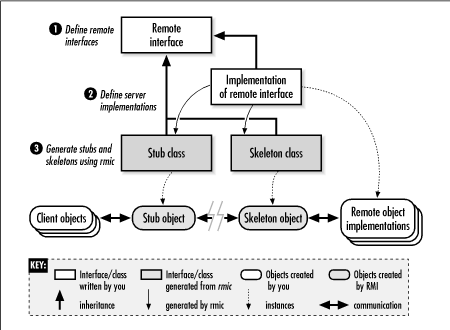
\includegraphics[width=150mm]{img/remote_object_relationship.png}
\caption{Relationships among remote object, stub, and skeleton classes}
\label{Remote Object relationship}
\end{figure}

\subsection{Remote Method Invocation}
The Java Remote Method Invocation system is a mechanism that enables an object on one Java virtual machine to invoke methods on an object in another Java virtual machine. Any object whose methods can be invoked in this way must implement the java.rmi.Remote interface. When such an object is invoked, its arguments are marshalled and sent from the local virtual machine to the remote one, where the arguments are \emph{unmarshalled} and used. When the method terminates, the results are \emph{marshalled} (meaning it must be serializeable) from the remote machine and sent to the caller's virtual machine.

To make a remote object accessible to other virtual machines, a program typically registers it with the RMI registry. The program supplies to the registry the string name of the remote object as well as the remote object itself. When a program wants to access a remote object, it supplies the object's string name to the registry that is on the same machine as the remote object. The registry returns to the caller a reference (called stub) to the remote object. When the program receives the stub for the remote object, it can invoke methods on the object (through the stub).